\documentclass[11pt,a4paper]{article}

\usepackage[a4paper,margin=18mm,headheight=16pt]{geometry}
\usepackage[T1]{fontenc}
\usepackage[scaled=0.94]{helvet}
\usepackage{inconsolata}
\renewcommand{\familydefault}{\sfdefault}

\usepackage{xcolor}
\definecolor{Ink}{HTML}{172033}
\definecolor{Muted}{HTML}{596579}
\definecolor{Blue}{HTML}{2855D9}
\definecolor{BlueLight}{HTML}{EEF3FF}
\definecolor{Amber}{HTML}{A86200}
\definecolor{AmberLight}{HTML}{FFF7E8}
\definecolor{Green}{HTML}{237A57}
\definecolor{Red}{HTML}{B42318}
\definecolor{Rule}{HTML}{D9DFEA}
\definecolor{Paper}{HTML}{F5F7FB}

\usepackage{microtype}
\usepackage{etoolbox}
\usepackage{needspace}
\usepackage{parskip}
\setlength{\parindent}{0pt}
\setlength{\parskip}{5pt plus 1pt}
\usepackage{enumitem}
\setlist[itemize]{leftmargin=5mm,itemsep=2pt,topsep=3pt}
\setlist[enumerate]{leftmargin=7mm,itemsep=3pt,topsep=3pt}

\usepackage{titlesec}
\titleformat{\section}{\Large\bfseries\color{Ink}}{\thesection}{0.7em}{}
\titleformat{\subsection}{\large\bfseries\color{Ink}}{\thesubsection}{0.65em}{}
\titlespacing*{\section}{0pt}{18pt}{7pt}
\titlespacing*{\subsection}{0pt}{13pt}{5pt}

\usepackage{booktabs,tabularx,array}
\newcolumntype{Y}{>{\raggedright\arraybackslash}X}
\renewcommand{\arraystretch}{1.25}

% ---------------------------------------------------------------------------
% Callout boxes.
% Three types only: key (blue), caution (amber), reference (grey).
% The title is set inline as the first line of the body -- no title bar. This
% keeps the boxes quiet and avoids the dark-on-dark title rendering that the
% default tcolorbox title bar produces when colframe is left unset.
% ---------------------------------------------------------------------------
\usepackage[most]{tcolorbox}
\tcbset{enhanced,boxrule=0pt,arc=1.5mm,left=4mm,right=4mm,top=3mm,bottom=3mm}

\newtcolorbox{keybox}[1][]{colback=BlueLight,colframe=BlueLight,
  borderline west={2pt}{0pt}{Blue},
  before upper={\ifstrempty{#1}{}{{\bfseries #1}\par\vspace{1pt}}}}
\newtcolorbox{warnbox}[1][]{colback=AmberLight,colframe=AmberLight,
  borderline west={2pt}{0pt}{Amber},
  before upper={\ifstrempty{#1}{}{{\bfseries #1}\par\vspace{1pt}}}}
\newtcolorbox{plainbox}[1][]{colback=Paper,colframe=Paper,
  borderline west={2pt}{0pt}{Rule},
  before upper={\ifstrempty{#1}{}{{\bfseries #1}\par\vspace{1pt}}}}

\usepackage{tikz}
\usetikzlibrary{arrows.meta,positioning,calc}
\tikzset{
  flow/.style={draw=Rule,fill=white,rounded corners=1.5mm,minimum height=13mm,
    minimum width=27mm,align=center,text=Ink,font=\small\bfseries,inner sep=2pt},
  primary/.style={flow,draw=Blue,fill=BlueLight},
  stage/.style={draw=Rule,fill=white,rounded corners=1.5mm,minimum height=8mm,
    minimum width=20mm,align=center,text=Ink,font=\scriptsize\bfseries,inner sep=1pt},
  arrow/.style={-{Latex[length=2.2mm]},line width=.9pt,draw=Blue},
  sub/.style={font=\scriptsize\bfseries,text=Muted}
}

\usepackage{fontawesome5}
\newcommand{\yes}{\textcolor{Green}{\faCheck}}
\newcommand{\no}{\textcolor{Red}{\faTimes}}

\usepackage{fancyhdr}
\pagestyle{fancy}
\fancyhf{}
\lhead{\small\color{Muted}Unity + GitHub Desktop Course Guide}
\rhead{\small\color{Muted}\thepage}
\renewcommand{\headrulewidth}{0.4pt}
\renewcommand{\headrule}{\hbox to\headwidth{\color{Rule}\leaders\hrule height \headrulewidth\hfill}}

\usepackage{xurl}
\usepackage[hidelinks]{hyperref}
\hypersetup{colorlinks=true,linkcolor=Blue,urlcolor=Blue}
\usepackage{bookmark}

\newcommand{\button}[1]{\tcbox[on line,colback=white,colframe=Rule,boxrule=.5pt,
  arc=1mm,left=1.5mm,right=1.5mm,top=.6mm,bottom=.6mm]{\small\bfseries #1}}
\newcommand{\pathbit}[1]{\texttt{#1}}

\begin{document}

% ---------------------------------------------------------------------------
% Title page
% ---------------------------------------------------------------------------
\begin{titlepage}
\pagecolor{Ink}
\color{white}
\vspace*{42mm}
{\fontsize{14}{17}\selectfont\bfseries COURSE WORKFLOW GUIDE\par}
\vspace{7mm}
{\fontsize{34}{39}\selectfont\bfseries Unity + GitHub Desktop\par}
\vspace{5mm}
{\fontsize{17}{22}\selectfont Organise, version, protect, and move your course work\par}
\vspace{16mm}
\begin{tcolorbox}[colback=white!8!Ink,colframe=white!18!Ink,boxrule=.6pt,arc=2mm]
\color{white}
\textbf{For beginners working independently across one or more computers.}\\[2mm]
This guide uses one course repository containing design notes, a proposal, three Unity
prototypes, and three evaluations.
\end{tcolorbox}
\vfill
{\large Semester 2, 2026\par}
\vspace{4mm}
{\small\color{Rule}Guide version 1.0\par}
\end{titlepage}
\nopagecolor
\color{Ink}

\tableofcontents
\clearpage

% ---------------------------------------------------------------------------
% ---------------------------------------------------------------------------
\section{Quick reference}

This page is a summary. If you are setting up for the first time, start at Section~3 and
come back here once your repository is working.

\begin{keybox}[The daily workflow]
\vspace{1mm}
\centering
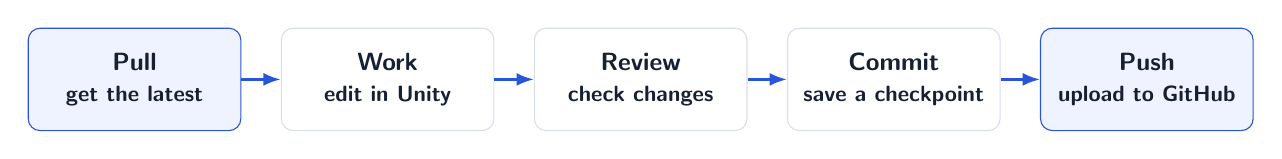
\begin{tikzpicture}[node distance=5mm]
\node[primary] (fetch) {Pull\\{\footnotesize get the latest}};
\node[flow,right=of fetch] (work) {Work\\{\footnotesize edit in Unity}};
\node[flow,right=of work] (review) {Review\\{\footnotesize check changes}};
\node[flow,right=of review] (commit) {Commit\\{\footnotesize save a checkpoint}};
\node[primary,right=of commit] (push) {Push\\{\footnotesize upload to GitHub}};
\draw[arrow] (fetch)--(work);
\draw[arrow] (work)--(review);
\draw[arrow] (review)--(commit);
\draw[arrow] (commit)--(push);
\end{tikzpicture}
\vspace{1mm}
\end{keybox}

\begin{minipage}[t]{0.48\textwidth}\vspace{0pt}
\begin{keybox}[Three essential rules]
\raggedright
\begin{enumerate}
\item Pull before beginning work.
\item Commit meaningful checkpoints.
\item Push before you leave or switch computers.
\end{enumerate}
\end{keybox}
\end{minipage}\hfill
\begin{minipage}[t]{0.48\textwidth}\vspace{0pt}
\begin{warnbox}[Large-file rule]
\raggedright
Normal GitHub repositories block individual files larger than 100~MiB. Keep builds,
long recordings, archives, caches, and other large generated files outside the
repository unless your course explicitly uses Git LFS.
\end{warnbox}
\end{minipage}

\begin{minipage}[t]{0.48\textwidth}\vspace{0pt}
\begin{keybox}[Before beginning]
\raggedright
\begin{itemize}[label={\faSquare[regular]}]
\item Open GitHub Desktop first
\item Fetch origin
\item Pull any available changes
\item Open the correct prototype
\item Confirm no unresolved conflicts
\end{itemize}
\end{keybox}
\end{minipage}\hfill
\begin{minipage}[t]{0.48\textwidth}\vspace{0pt}
\begin{plainbox}[Before finishing]
\raggedright
\begin{itemize}[label={\faSquare[regular]}]
\item Save and close Unity
\item Review changed files
\item Exclude large/generated files
\item Commit with a useful summary
\item Push origin
\item Confirm repository is up to date
\end{itemize}
\end{plainbox}
\end{minipage}

\clearpage
% ---------------------------------------------------------------------------
\section{What GitHub is doing}

GitHub gives your work a history. A \textbf{commit} saves a named checkpoint on your
computer. A \textbf{push} sends those commits to the online repository. A \textbf{pull}
retrieves newer commits from GitHub.

\begin{center}
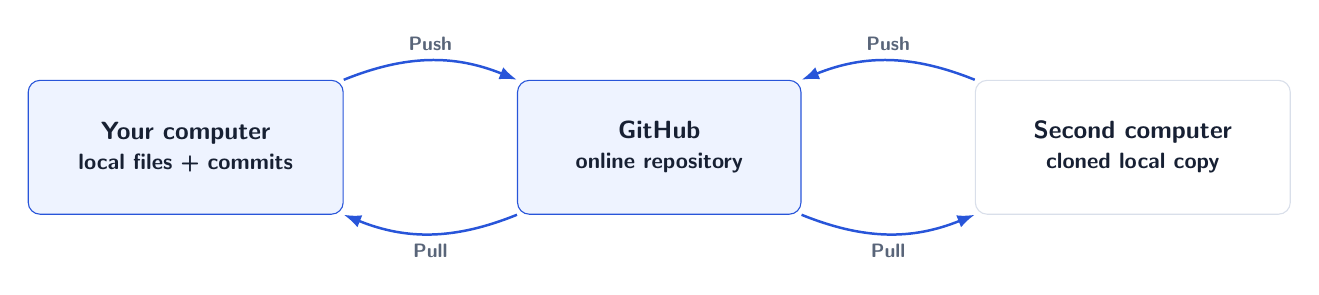
\begin{tikzpicture}
\node[primary,minimum width=40mm,minimum height=17mm] (a)
  {Your computer\\{\footnotesize local files + commits}};
\node[primary,right=22mm of a,minimum width=36mm,minimum height=17mm] (hub)
  {GitHub\\{\footnotesize online repository}};
\node[flow,right=22mm of hub,minimum width=40mm,minimum height=17mm] (b)
  {Second computer\\{\footnotesize cloned local copy}};
\draw[arrow] (a.north east) to[bend left=22] node[sub,above]{Push} (hub.north west);
\draw[arrow] (hub.south west) to[bend left=22] node[sub,below]{Pull} (a.south east);
\draw[arrow] (b.north west) to[bend right=22] node[sub,above]{Push} (hub.north east);
\draw[arrow] (hub.south east) to[bend right=22] node[sub,below]{Pull} (b.south west);
\end{tikzpicture}
\end{center}

\begin{center}
\begin{tabularx}{0.94\textwidth}{>{\bfseries}p{24mm}Y}
\toprule
Term & Meaning\\
\midrule
Repository & A project folder plus its Git version history.\\
Commit & A named checkpoint saved in the local repository.\\
Push & Upload local commits to GitHub.\\
Fetch & Check GitHub for newer commits without changing local files.\\
Pull & Download and apply newer commits from GitHub.\\
Clone & Download a repository to a computer for the first time.\\
\bottomrule
\end{tabularx}
\end{center}

\begin{keybox}[Sections 3 to 7 are done once]
Sections~3--7 set everything up and finish with your first commit. After that you repeat
the short loop in Section~10 for the rest of the course.
\end{keybox}

% ---------------------------------------------------------------------------
\section{Before you start}

Install these three things and sign in before creating anything. Publishing a repository
later will not work until you are signed into GitHub Desktop.

\subsection{Create a GitHub account}
\begin{enumerate}
\item Go to \url{https://github.com} and create a free account if you do not already have
one.
\item Use an email address you will keep for the whole course.
\item Verify that email address. GitHub will not let you publish work until you do.
\end{enumerate}

\subsection{Install GitHub Desktop and sign in}
\begin{enumerate}
\item Download GitHub Desktop from \url{https://desktop.github.com} and install it.
\item Open it and sign in with the GitHub account you just created.
\item Check that your name and email are filled in, under
\button{File} $>$ \button{Options} $>$ \button{Git} on Windows, or
\button{GitHub Desktop} $>$ \button{Settings} $>$ \button{Git} on macOS. These appear on
every commit you make.
\end{enumerate}

\subsection{Install Unity Hub and the Editor}
\begin{enumerate}
\item Install Unity Hub and sign in with a Unity account.
\item Install the Unity Editor version specified for the course, and use that version for
every prototype.
\end{enumerate}

\begin{warnbox}[Use the version the course specifies]
Opening a project in a newer Editor upgrades it, and the upgrade cannot be undone by
pulling. If you and a lab computer use different versions, the project can break when
work moves between them.
\end{warnbox}

% ---------------------------------------------------------------------------
\section{Create the course repository}

You will create the repository first, as an empty folder, and then build everything else
inside it.

\begin{enumerate}
\item Open GitHub Desktop.
\item Select \button{File} $>$ \button{New repository}.
\item For \textbf{Name}, enter \pathbit{XR-YourName}. This name becomes the folder name.
\item For \textbf{Local path}, choose where the folder should live, such as your
Documents folder. GitHub Desktop creates the repository folder inside that location.
\item Leave \textbf{Git ignore} set to \texttt{None}. You will install the supplied course
file in Section~5.
\item Select \button{Create repository}.
\end{enumerate}

You now have one folder that is a Git repository. Everything for the course goes inside
it.

\begin{warnbox}[One repository, at the top]
Create this repository once. Do not create a second repository inside
\pathbit{Prototype1}, inside \pathbit{Assets}, or for each prototype, unless your teaching
team explicitly instructs you to.
\end{warnbox}

% ---------------------------------------------------------------------------
\section{Install the supplied \texttt{.gitignore}}

Download the supplied \pathbit{.gitignore} and place it directly inside the repository
folder you just created, before you create any Unity project.

A \pathbit{.gitignore} tells Git which files to leave alone. Unity generates a very large
amount of temporary data that it can rebuild at any time, and none of it belongs on
GitHub.

\begin{plainbox}[What this file prevents]
Without it, opening a Unity project inside the repository would leave GitHub Desktop
showing something like:
\begin{verbatim}
  Library/Bee/artifacts/...          ~ several thousand changed files
  Library/PackageCache/...
  Library/ShaderCache/...
  Temp/...
  Logs/...
\end{verbatim}
None of that is your work. With the file installed, you will see three folders instead.
\end{plainbox}

\begin{warnbox}[Check the filename]
\yes~\textbf{Correct:} \pathbit{.gitignore}\qquad
\no~\textbf{Incorrect:} \pathbit{.gitignore.txt}

On Windows, enable file-name extensions in File Explorer before checking. The leading dot
is part of the filename.
\end{warnbox}

The supplied version is designed for a repository containing several nested Unity
projects. It recursively ignores generated Unity folders, IDE metadata, builds, logs, test
output, archives, and common operating-system files.

% ---------------------------------------------------------------------------
\section{Create your first Unity project}

The first prototype is created \textbf{inside} the repository folder, in a subfolder named
\pathbit{Prototype1}. The full course layout comes later, in Section~8.

\begin{enumerate}
\item Open Unity Hub and select \button{New project}.
\item Choose the Editor version and template required by the course.
\item Set \textbf{Project name} to \pathbit{Prototype1}.
\item Set \textbf{Location} to your repository folder, so the project is created at
\pathbit{XR-YourName/Prototype1}.
\item Create the project and wait for Unity to finish its first import.
\item Confirm that \pathbit{Prototype1} now contains \pathbit{Assets},
\pathbit{Packages}, and \pathbit{ProjectSettings}.
\end{enumerate}

\begin{warnbox}[Inside, not beside]
If Unity Hub creates the project next to the repository folder rather than inside it, Git
cannot see the project at all. Check the path before selecting \button{Create project}.
\end{warnbox}

% ---------------------------------------------------------------------------
\section{Your first commit}

This section is the loop you will repeat for the rest of the course. Do it once now, with
a small amount of work, so the steps are familiar.

\subsection{Review what Git can see}
Switch back to GitHub Desktop. It should list a short set of changes: the
\pathbit{.gitignore} and the three Unity folders that matter.

\begin{keybox}[Expected changes]
\pathbit{.gitignore}\quad \pathbit{Prototype1/Assets/}\quad
\pathbit{Prototype1/Packages/}\quad \pathbit{Prototype1/ProjectSettings/}

This short list is the \pathbit{.gitignore} doing its job. Without it, the same screen
would be listing several thousand generated files.
\end{keybox}

\begin{warnbox}[Stop if generated files appear]
If GitHub Desktop shows thousands of files inside \pathbit{Library}, do not commit. The
\pathbit{.gitignore} is missing, incorrectly named, or in the wrong folder. Fix it before
going any further — removing these files after they are committed is much harder.
\end{warnbox}

\subsection{Commit and publish}
\begin{enumerate}
\item Enter a summary describing what you did, such as
\texttt{Set up course repository and Prototype 1}.
\item Select \button{Commit to main}.
\item Select \button{Publish repository}.
\item Keep the repository private unless the course explicitly requires a public one.
\item Open the repository on \url{https://github.com} and confirm your files are there.
\end{enumerate}

\begin{keybox}[You have now done the whole loop]
Review the changes, commit them with a useful summary, push them to GitHub. That is the
loop, and it does not get more complicated than this. Section~10 covers when to run it.
\end{keybox}

% ---------------------------------------------------------------------------
\section{Organising the course repository}

Your repository currently holds one prototype. Add the remaining folders now so there is
an obvious place for every piece of work.

\begin{center}
\begin{minipage}{0.72\textwidth}
\begin{plainbox}
\begin{verbatim}
XR-YourName/
|-- README.md
|-- .gitignore
|-- DesignNotes/
|   |-- Notes/
|   |-- Sketches/
|   `-- Images/
|-- Proposal/
|-- Prototype1/
|   |-- Assets/
|   |-- Packages/
|   `-- ProjectSettings/
|-- Evaluation1/
|-- Prototype2/        (same three folders)
|-- Evaluation2/
|-- Prototype3/        (same three folders)
`-- Evaluation3/
\end{verbatim}
\end{plainbox}
\end{minipage}
\end{center}

\subsection{What belongs in each folder}

\begin{tabularx}{\textwidth}{>{\bfseries}p{32mm}Y}
\toprule
DesignNotes & Raw notes, ideas, sketches, screenshots, observations, useful links, and
working thoughts from across the course. This is flexible working material, not a
separate journal.\\
Proposal & The initial design proposal and any supporting material required for it.\\
Prototype1--3 & Each folder is a complete, self-contained Unity project. Its root
contains \pathbit{Assets}, \pathbit{Packages}, and \pathbit{ProjectSettings}.\\
Evaluation1--3 & The testing plan, results, and supporting evidence for the prototype
immediately before it. Keep this explanation brief and follow the assessment
instructions for the required contents.\\
README.md & A short identification page containing the course, student name, and a
summary of the repository.\\
.gitignore & Rules telling Git which generated, temporary, build, and local files must
not be tracked.\\
\bottomrule
\end{tabularx}

\subsection{Add them and commit}
\begin{enumerate}
\item Create \pathbit{DesignNotes}, \pathbit{Proposal}, and the numbered evaluation
folders inside the repository.
\item Add a short \pathbit{README.md} naming the course and yourself.
\item Create \pathbit{Prototype2} and \pathbit{Prototype3} in Unity Hub when the course
reaches them, using the same method as Section~6.
\item Run the loop again: review, commit with a summary such as
\texttt{Add course folder structure}, and push.
\end{enumerate}

\begin{plainbox}[Git does not track empty folders]
A folder with nothing in it will not appear in GitHub Desktop. This is normal. It will
show up as soon as you put a file in it.
\end{plainbox}

% ---------------------------------------------------------------------------
\section{What to keep out of Git}

Large-file mistakes are among the easiest ways to make a beginner repository difficult or
impossible to push. Check file size \textbf{before} committing large media or exported
applications.

\begin{warnbox}[GitHub's normal file limit]
GitHub warns when a normal Git repository contains a file larger than 50~MiB and blocks
files larger than 100~MiB. Git LFS can store files beyond the normal limit, but it
introduces quotas and should only be used when the course requires it.
\end{warnbox}

\begin{tabularx}{\textwidth}{>{\raggedright\arraybackslash}p{40mm}>{\centering\arraybackslash}p{20mm}Y}
\toprule
\textbf{Item} & \textbf{Track?} & \textbf{Reason}\\
\midrule
\pathbit{Assets} & Yes & Scripts, scenes, prefabs, materials, models, and required
project content.\\
\pathbit{Packages} & Yes & Records the packages required by the project.\\
\pathbit{ProjectSettings} & Yes & Records Unity project configuration.\\
Design notes and proposal & Yes & Part of the course work and its history.\\
Testing plans and results & Yes & Part of each evaluation record.\\
Small evidence images & Yes & Genuinely part of the project record.\\
\midrule
\pathbit{Library} & No & Large generated cache that Unity recreates.\\
\pathbit{Temp}, \pathbit{Logs} & No & Temporary and diagnostic files.\\
Builds and exported apps & No & Large generated outputs that can be rebuilt.\\
ZIP archives and backups & No & Whole-project copies do not belong in a repository that
already keeps history.\\
Duplicated or unused media & No & High-resolution source files nothing references.\\
Package installers & No & Platform and build artefacts.\\
Long videos and raw footage & Usually no & Store in the location specified in your
assessment task sheet.\\
\bottomrule
\end{tabularx}

% ---------------------------------------------------------------------------
\section{The daily workflow}

\subsection{Start of a session}
\begin{enumerate}
\item Open GitHub Desktop before Unity.
\item Select the course repository.
\item Select \button{Fetch origin}.
\item If GitHub Desktop reports remote changes, select \button{Pull origin}.
\item Only then open the required prototype in Unity Hub.
\end{enumerate}

\begin{keybox}[Why fetch comes first]
\textbf{Fetch} checks whether GitHub contains newer commits. \textbf{Pull} downloads and
applies them. Starting with this check prevents you from editing an older copy of the
project.
\end{keybox}

\Needspace{12\baselineskip}
\subsection{During a session}
Commit at meaningful checkpoints. A commit should describe a change you may later want to
identify or restore.

\begin{plainbox}[Commit summaries]
\raggedright
\begin{tabularx}{\linewidth}{YY}
\yes~\textbf{Useful} & \no~\textbf{Unhelpful}\\
\midrule
Add teleport interaction & stuff\\
Build first menu layout & changes\\
Fix grabbing on small objects & final final\\
Prepare Prototype 2 for testing & asdf\\
\end{tabularx}
\end{plainbox}

\subsection{End of a session}
\begin{enumerate}
\item Save your Unity scenes and project.
\item Close Unity so it finishes writing project files.
\item Review the changed files in GitHub Desktop.
\item Confirm that no large, generated, or unrelated files are included.
\item Write a meaningful commit summary.
\item Select \button{Commit to main}.
\item Select \button{Push origin}.
\item Confirm GitHub Desktop reports that the branch is up to date.
\end{enumerate}

% ---------------------------------------------------------------------------
\section{Moving between computers}

Finish and push on one computer, then pull on the other. The steps are the ordinary start
and end of a session from Section~10.

\begin{center}
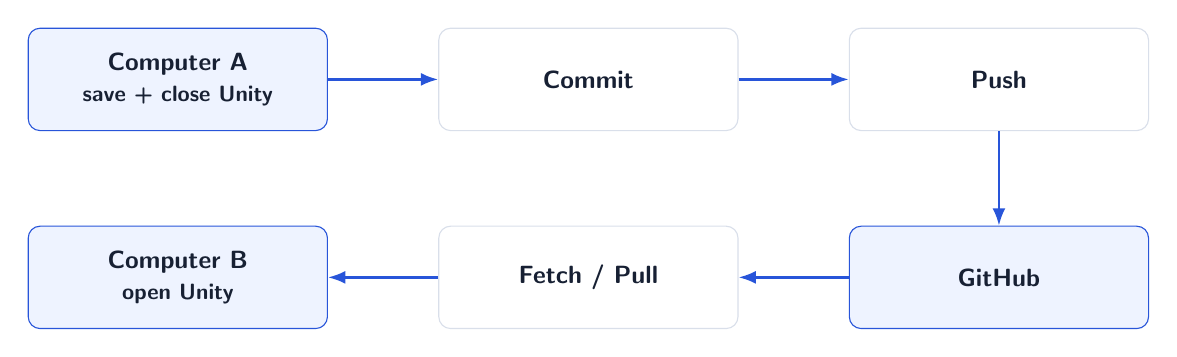
\begin{tikzpicture}[node distance=14mm]
\node[primary,minimum width=38mm] (a) {Computer A\\{\footnotesize save + close Unity}};
\node[flow,right=of a,minimum width=38mm] (c) {Commit};
\node[flow,right=of c,minimum width=38mm] (p) {Push};
\node[primary,below=12mm of p,minimum width=38mm] (g) {GitHub};
\node[flow,left=of g,minimum width=38mm] (f) {Fetch / Pull};
\node[primary,left=of f,minimum width=38mm] (b) {Computer B\\{\footnotesize open Unity}};
\draw[arrow] (a)--(c);
\draw[arrow] (c)--(p);
\draw[arrow] (p)--(g);
\draw[arrow] (g)--(f);
\draw[arrow] (f)--(b);
\end{tikzpicture}
\end{center}

\subsection{Setting up a computer that has never had the repository}
\begin{enumerate}
\item Install GitHub Desktop, Unity Hub, and the required Unity Editor version, as in
Section~3.
\item Sign into GitHub Desktop.
\item Select \button{Clone a repository} and choose the course repository.
\item Choose a suitable local location.
\item In Unity Hub, add the required \pathbit{Prototype1}, \pathbit{Prototype2}, or
\pathbit{Prototype3} folder as a project.
\item Allow Unity to recreate its generated \pathbit{Library} files. The first opening
may take time.
\end{enumerate}

\begin{warnbox}[Do not work on both copies at once]
Do not keep the same project open and make independent edits on two computers. Finish,
commit, and push on one computer before pulling and continuing on the other.
\end{warnbox}

% ---------------------------------------------------------------------------
\section{Common problems}

\subsection*{Publish repository does not work}
Check that you are signed into GitHub Desktop and that you have verified your GitHub email
address. Both are covered in Section~3.

\subsection*{My latest work is missing}
Check whether the previous computer committed \textbf{and pushed} the work. Then fetch and
pull on the current computer. A local commit that was never pushed cannot appear on
another device.

\subsection*{Unity is importing everything}
This is expected after cloning or opening the project on a new computer. Unity is
recreating the ignored \pathbit{Library} folder.

\subsection*{GitHub Desktop shows thousands of generated files}
Stop before committing. Check that the file is named exactly \pathbit{.gitignore} and sits
at the top of the repository, beside \pathbit{Prototype1} rather than inside it.

\subsection*{A file is too large to push}
Do not repeatedly retry. Remove the file from the commit and move it to the location
specified in your assessment task sheet. Adding a filename to \pathbit{.gitignore} after
it has already been committed does not automatically remove it from Git history; ask the
teaching team for help.

\subsection*{GitHub reports a merge conflict}
Stop editing and do not choose conflict-resolution options at random. Preserve a copy of
your current work and ask the teaching team for help.

% ---------------------------------------------------------------------------
\section*{Appendix: authoritative references}
\addcontentsline{toc}{section}{Appendix: authoritative references}

\begin{itemize}
\item GitHub's maintained Unity ignore template:\\
\url{https://github.com/github/gitignore/blob/main/Unity.gitignore}
\item GitHub documentation for large files:\\
\url{https://docs.github.com/en/repositories/working-with-files/managing-large-files}
\item Git LFS and GitHub Desktop:\\
\url{https://docs.github.com/en/desktop/configuring-and-customizing-github-desktop/about-git-large-file-storage-and-github-desktop}
\end{itemize}

\end{document}
